%%%%%%%%%%%%%%%%%%%%%%%%%%%%%%%%%%%%%%%%%%%%%%%%%%%%%%%%%%%%%%%%%%
%  = PREAMBLE =
% The preamble of a LaTeX document is the set of commands that 
%    precede the \begin{document} line.  It sets up the style of 
%    the document.
%%%%%%%%%%%%%%%%%%%%%%%%%%%%%%%%%%%%%%%%%%%%%%%%%%%%%%%%%%%%%%%%%%

\documentclass[aps,twocolumn, secnumarabic,balancelastpage,amsmath,amssymb,nofootinbib,floatfix]{revtex4-1}

\usepackage{graphicx}      % tools for importing graphics
\usepackage{parskip}
\usepackage[colorlinks=true]{hyperref}  % this package should be added after 
                                        % all others.
                                        % usage: \url{http://web.mit.edu/8.13}

%%%%%%%%%%%%%%%%%%%%%%%%%%%%%%%%%%%%%%%%%%%%%%%%%%%%%%%%%%%%%%%%%%%
% And now, begin the document...
%%%%%%%%%%%%%%%%%%%%%%%%%%%%%%%%%%%%%%%%%%%%%%%%%%%%%%%%%%%%%%%%%%%

\begin{document}

\title{Michelson Experiment Summary}
\author{Yongao Hu}
\email{yongao@mit.edu}
\date{\today}
\affiliation{MIT Department of Physics}


\begin{abstract}
The summary reports the results of the Michelson interferometer experiment conducted in MIT Junior Lab Spring 2025. The experiment was conducted to measure the wavelength of the light source. The wavelength of the laser was found to be $601\pm37(\text{sys})\pm10(\text{stat})\text{ nm}$. The experiment was successful in demonstrating the principles of interference and the wave nature of light.
\end{abstract}

\maketitle

\section{Introduction}
Michelson interferometer is designed by Albert Michelson to measure the wavelength of light \cite{MichelsonMorley1887}. The interferometer is based on the principle of interference of light waves. The experiment was conducted to measure the wavelength of the light source. 

The Michelson interferometer consists of a beam splitter, two mirrors, and a detector \cite{MichelsonMorley1887,MITOpticalInterferometry2023}. The beam splitter splits the light beam into two beams. The two beams travel different paths and are reflected back by the mirrors. The two beams are then recombined at the beam splitter. The interference pattern is detected by the detector. 

\section{Theory}
The Michelson interferometer is based on the principle of interference of waves. The interference pattern is determined by the phase difference between the two waves. For two waves of the same wavelength $\lambda$, the phase difference is given by $\Delta \phi = 2\pi \frac{\Delta x}{\lambda}$, where $\Delta x$ is the path difference between the two waves. The interference pattern is given by $I = I_0 \cos^2(\Delta \phi)$, where $I_0$ is the intensity of the light source.

In order to change the path difference $\Delta x$, we use a piezoelectric transducer to move one of the mirrors \cite{MITOpticalInterferometry2023}. Piezoelectric transducer is an electronic device that changes its shape when a voltage is applied \cite{PiezoFilm2006}. The piezoelectric device we are using in particular changes its length when voltage is applied, moving the mirror by length $\Delta L$.  The change in length is proportional to the voltage applied \cite{MITOpticalInterferometry2023}. 

When we apply different voltage to the piezoelectric device, we change the path difference $\Delta x$ between the two waves, changing the interference pattern as a result. By recording what voltage corresponds to the maximum and minimum of the interference pattern, we can find the average $\Delta V$ between consequtive maximum and minimum. The wavelength of the light source is then given by:
\begin{equation}
    \lambda = 4 \Delta V \times \frac{\Delta L}{V} 
\end{equation}

Moreover, we record the intensity of the light source at different voltages to find the visibility of the interference pattern. The visibility is given by:
\begin{equation}
    V = \frac{I_{\text{max}} - I_{\text{min}}}{I_{\text{max}} + I_{\text{min}}}
\end{equation}
where $I \propto V_{\text{diode}}$. 


\section{Experiment}
The experiment was conducted using the Michelson interferometer setup in MIT Junior Lab in Feburary 2025 \cite{MITOpticalInterferometry2023}. The light source is a laser. The beam splitter was a 50/50 beam splitter. One mirror is stationary, while the other mirror is mounted on a piezoelectric transducer. The piezoelectric device we use is calibrated to have the length-voltage ratio of:
\begin{equation}
     \frac{\Delta L}{V} = 47.1\pm2.9 \text{ nm/V}
\end{equation}
The detector is a photodiode. The voltage output of photodiode is proportional to the intensity of the light on the detector. We used a signal generator to apply a triangular voltage of amplitude of $10 \text{ V}$ and frequency of $10 \text{ Hz}$ to the piezoelectric transducer. The schematic of the setup is shown in Fig. \ref{fig:set_up}.

The voltage was then applied to change the path difference $\Delta x$. We recorded the signal generator voltage and the photodiode voltage. 
\begin{figure}[h]
    \centering
    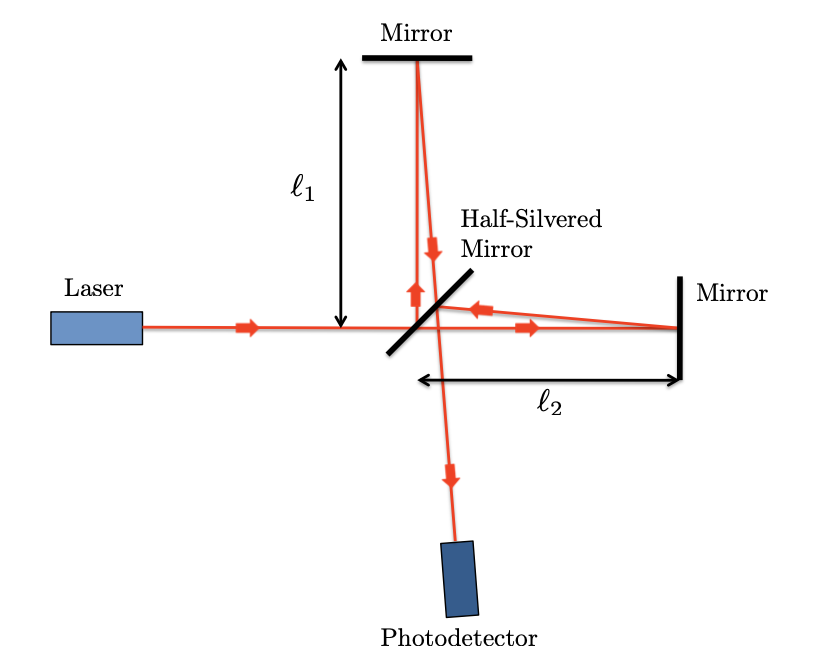
\includegraphics[width=0.45\textwidth]{fig/michelson_setup.png}
    \caption{The set up of the Michelson interferometer. The figure is reproduced from \cite{MITOpticalInterferometry2023}.}
    \label{fig:set_up}
\end{figure}

\section{Data Analysis}
We obtained the data from the output of the oscilloscope. We recorded the voltage of the signal generator and the voltage of the photodiode. We then used the \texttt{findpeak} function of \texttt{SciPy} to find the principle maxima and minima of the photodiode voltage. In order to filter out the secondary maxima and minima that occurs when the triangular input voltage changes direction, we chose the prominence of the peaks to be $0.4$.

The voltages of the signal generator at principle maxima and minima are shown in Fig. \ref{fig:data}. 
\begin{figure}[h]
    \centering
    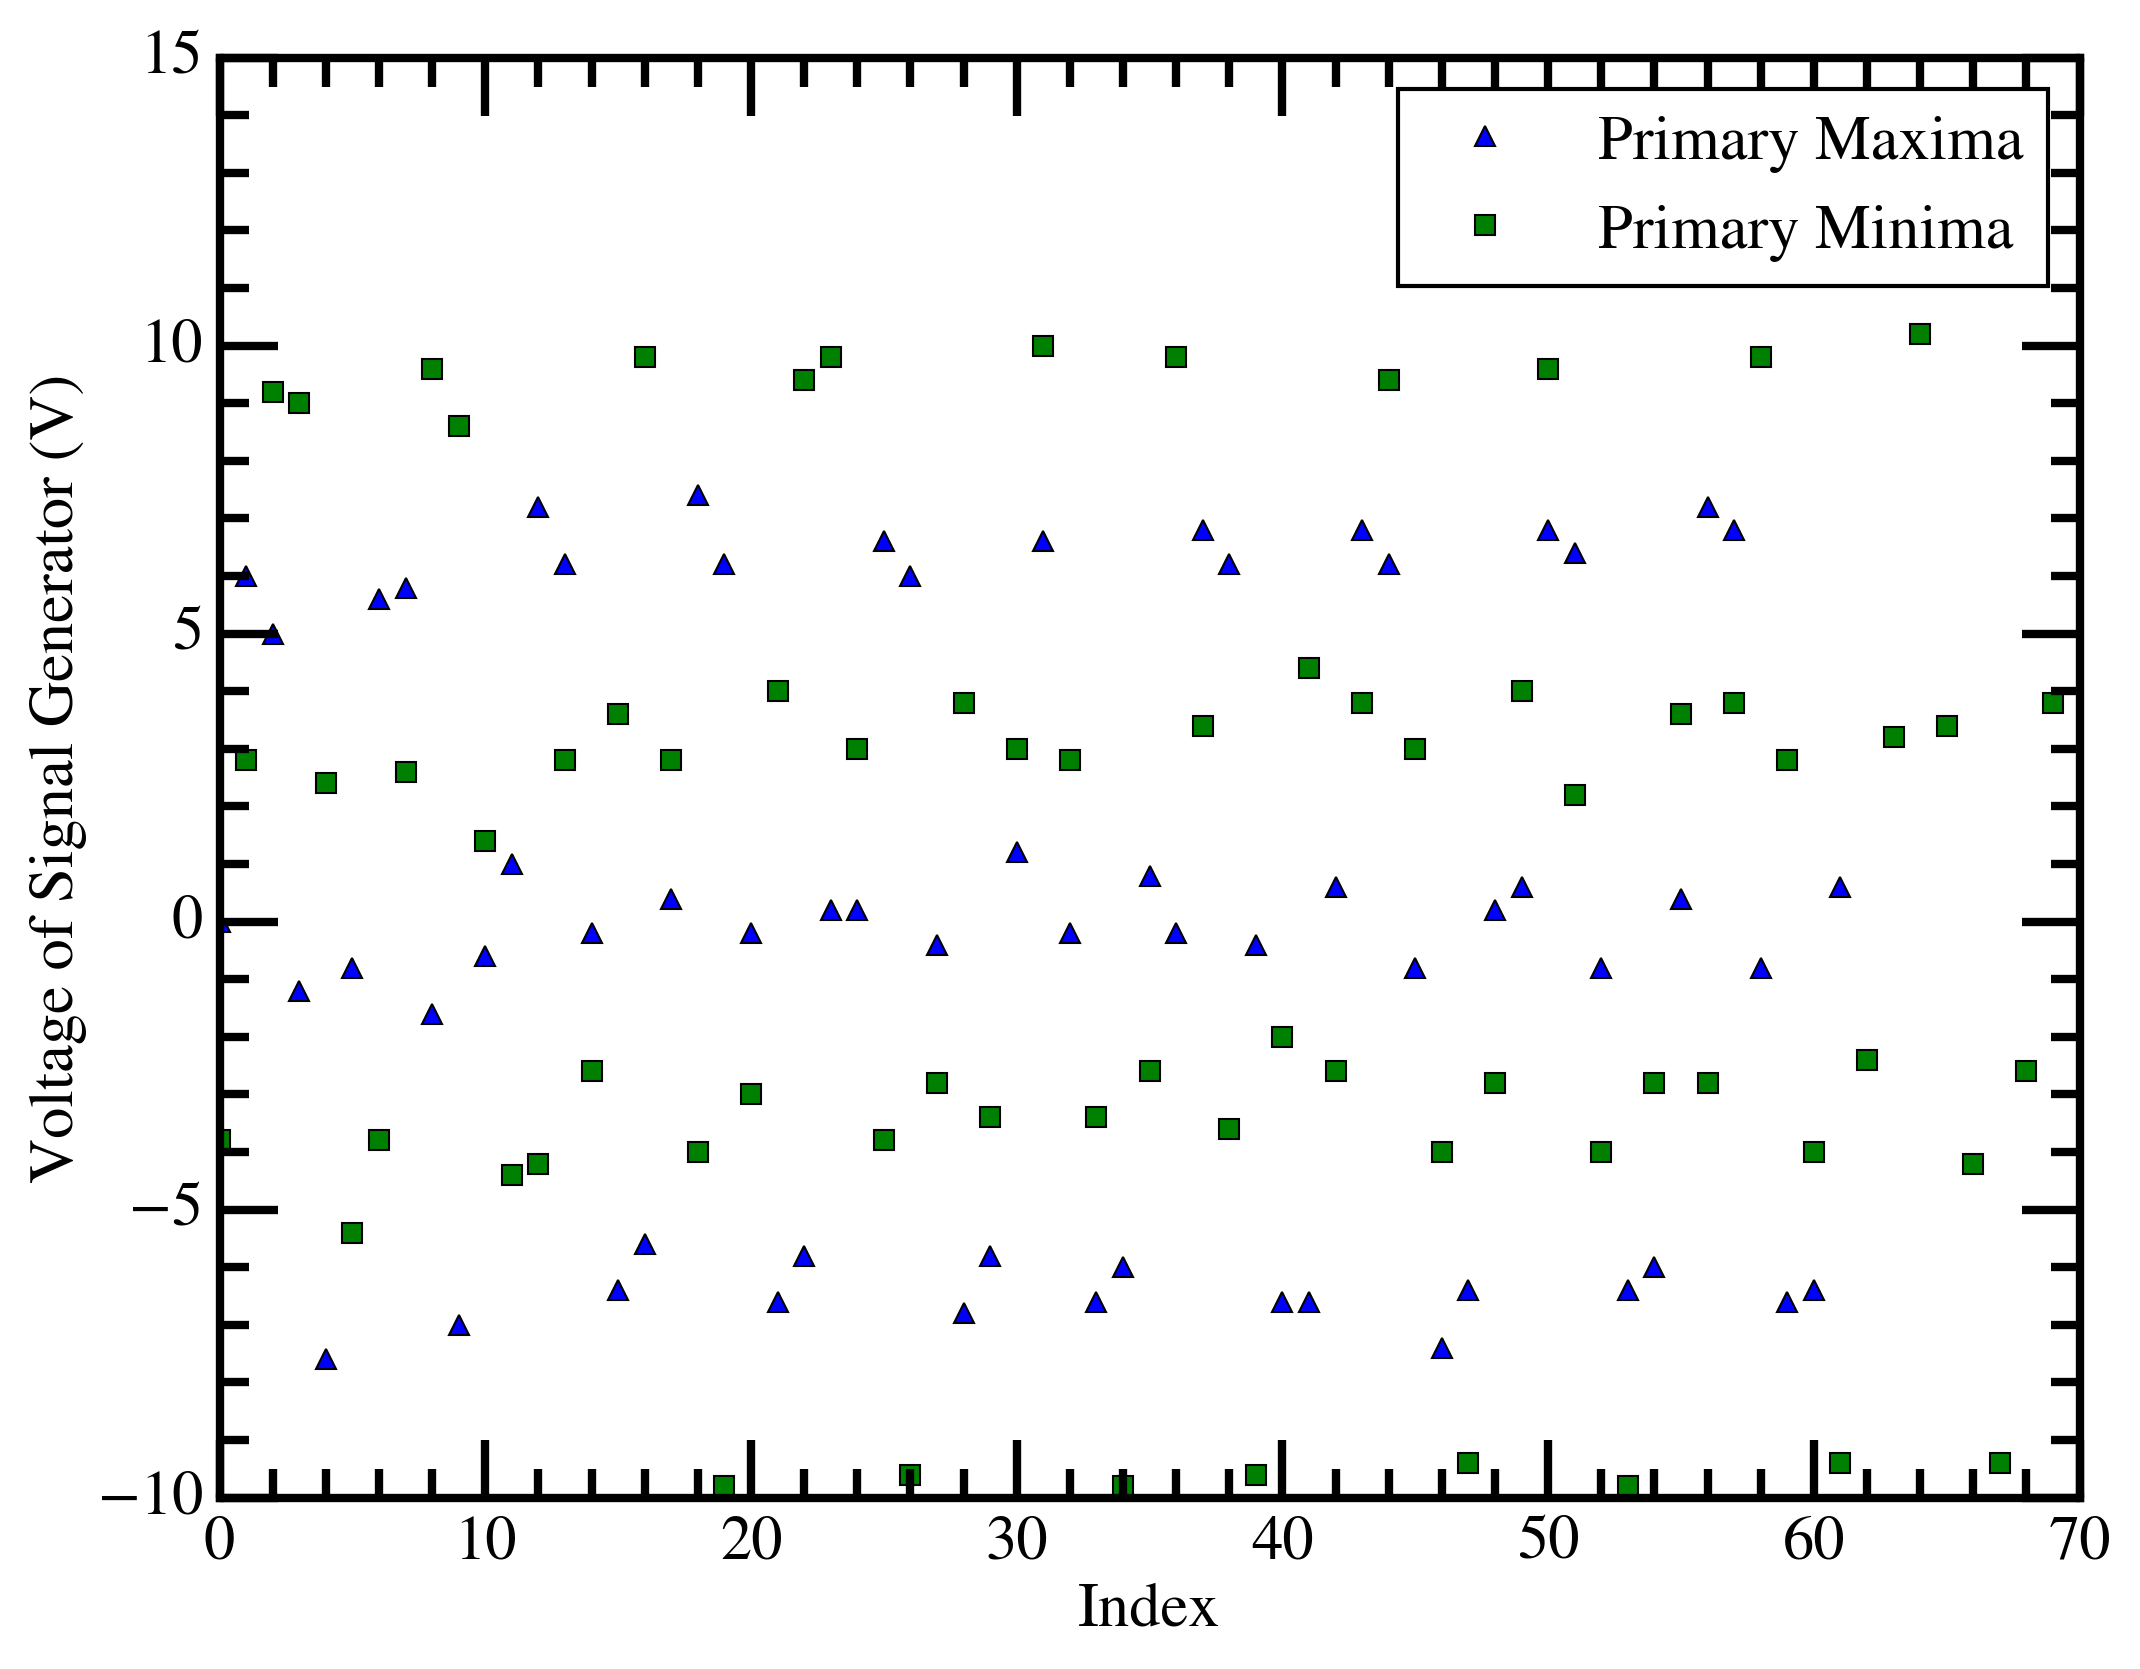
\includegraphics[width=0.5\textwidth]{fig/Primary_Maxima_Minima.png}
    \caption{The primary maxima and minima of the interference pattern.}
    \label{fig:data}
\end{figure}

In order to cluster the different bands of signal generator voltage to find the neighboring principle maxima and minima, we used the \texttt{KMeans} clustering algorithm of \texttt{SciKit-Learn}. 

The clustering algorithm identified 3 clusters of principle maxima and 4 clusters of principle minima. 

\section{Results}


\begin{acknowledgments} The author gratefully acknowledges J. Lewis and M. Bohdan for their invaluable help in conducting the experiment. The author also acknowledges their lab partner V. Tran for their invaluable help in data analysis. The author also thanks the teaching assistant for their guidance in the lab. This work was supported by the MIT Department of Physics. 
\end{acknowledgments}


\bibliographystyle{abbrv}
\bibliography{report_michelson_ref}
\end{document}

